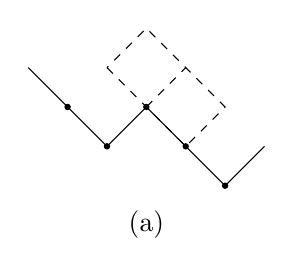
\begin{tikzpicture}
[scale = .5, dot/.style ={draw,shape=circle, fill=black, scale=.2}]
\draw (0,0) -- (1,-1) node[dot]{} -- (2,-2) node[dot]{} -- (3,-1) node[dot]{} --
      (4,-2) node[dot]{} -- (5,-3) node[dot]{} -- (6,-2);
\draw[dashed] (2,0) -- (4,-2) -- (5,-1) -- (3,1) -- (2,0) (3,-1) -- (4,0);
\draw (3,-4) node{(a)};
\end{tikzpicture}
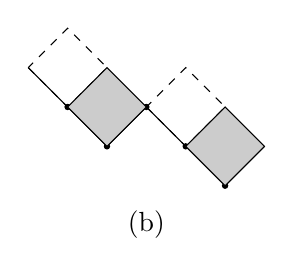
\begin{tikzpicture}
[scale = .5, dot/.style ={draw,shape=circle, fill=black, scale=.2}]
\draw (0,0) -- (1,-1) node[dot]{} -- (2,-2) node[dot]{} -- (3,-1) node[dot]{} --
(4,-2) node[dot]{} -- (5,-3) node[dot]{} -- (6,-2);
\draw[dashed] (0,0) -- (1,-1) -- (2,0) -- (1,1) -- (0,-0);
\draw[fill=black!20] (1,-1) -- (2,-2) -- (3,-1) -- (2,0) -- (1,-1);
\draw[dashed] (3,-1) -- (4,-2) -- (5,-1) -- (4,0) -- (3,-1);
\draw[fill=black!20] (4,-2) -- (5,-3) -- (6,-2) -- (5,-1) -- (4,-2);
\draw (3,-4) node{(b)};
\end{tikzpicture}
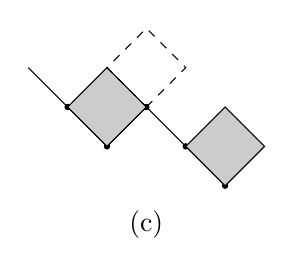
\begin{tikzpicture}
[scale = .5, dot/.style ={draw,shape=circle, fill=black, scale=.2}]
\draw (0,0) -- (1,-1) node[dot]{} -- (2,-2) node[dot]{} -- (3,-1) node[dot]{} --
(4,-2) node[dot]{} -- (5,-3) node[dot]{} -- (6,-2);
\draw[fill=black!20] (1,-1) -- (2,-2) -- (3,-1) -- (2,0) -- (1,-1);
\draw[dashed] (3,-1) -- (4,0) -- (3,1) -- (2,0) -- (3,-1);
\draw[fill=black!20] (4,-2) -- (5,-1) -- (6,-2) -- (5,-3) -- (4,-2);
\draw (3,-4) node{(c)};
\end{tikzpicture}